% For some reason pdflatex says it can't find this file, then i type "X" and it works
% also you have to compile it twice to get the png
\documentclass[preview, convert={density=300,size=1080x800,outext=.png}]{standalone}
\usepackage{tikz}
\usepackage{tkz-graph}

\SetVertexNormal[Shape      = circle,
                 FillColor  = orange,
                 LineWidth  = 2pt]
\SetUpEdge[lw         = 0.5pt,
           color      = black,
           labelcolor = white,
           labeltext  = red]


\begin{document}
\begin{figure}
    \centering
    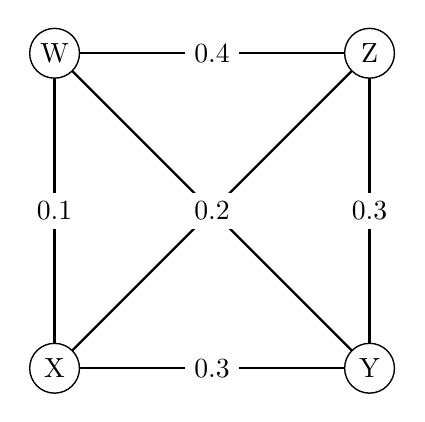
\begin{tikzpicture}
        \Vertex[ x=0, y=0]{X}
        \Vertex[ x=4, y=0]{Y}
        \Vertex[ x=4, y=4]{Z}
        \Vertex[ x=0, y=4]{W}

        \Edge[label=0.1](X)(W)
        \Edge[label=0.3](X)(Y)
        \Edge[label=0.2](X)(Z)
        \Edge[label=0.2](Y)(W)
        \Edge[label=0.3](Y)(Z)
        \Edge[label=0.4](Z)(W)
    \end{tikzpicture}
\end{figure}
\end{document}
